\section{Einführung und Überblick}
\subsection{Was ist Reinforcement Learning?}
Reinforcement Learning (dt.\ Verstärkendes Lernen) beschäftigt sich mit der 
Frage, wie man autonomen Agenten, die mit ihrer Umgebung interagieren, 
beibringt, optimale Entscheidungen zu treffen um so ihre Ziele zu erreichen.

\subsection{Grundlagen des Reinforcement Learnings}
Das Reinforcement Learning funktioniert nach dem Prinzip "`Zuckerbrot und 
Peitsche"'. Ein Agent, der sich in einem ihm unbekannten Zustandsraum befindet, 
bekommt für jede Aktion die er ausführt, eine Belohnung oder Bestrafung 
(Reward). Anhand dieser versucht er eine optimale Handlungsstrategie zu finden, 
das heißt eine Strategie (Policy), die die Belohnung maximiert. Was man bei 
Reinforcement Learning letztlich also sucht, ist eine \textbf{optimale 
Strategie $\Pi^*$}.

\begin{figure}
  \centering
  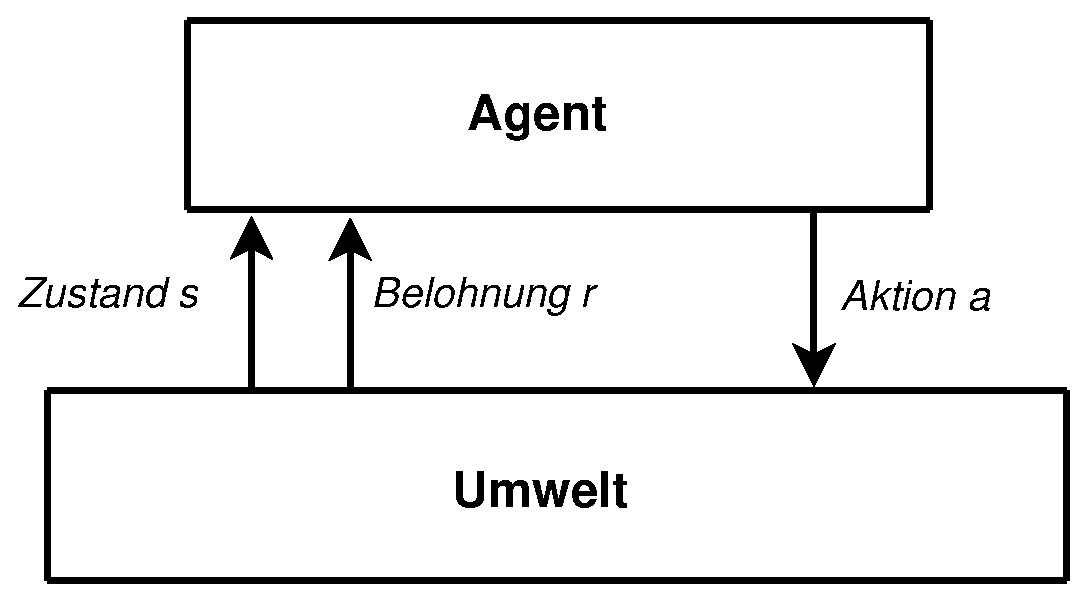
\includegraphics[width=0.5\textwidth]{../images/Agent_Umwelt.eps}
  \caption{Schema des typischen Reinforcement-Szenarios}
\end{figure}

\par Wir beschränken uns dabei hier auf einen diskreten Zustandsraum mit einer 
endlichen Anzahl von Aktionen in jedem Zustand. Hierbei wird auch zwischen zwei 
Fällen unterschieden, dem indeterministischen und dem deterministischen Fall. 
Auf letzterem, dem deterministischen Fall, liegt im Rahmen dieser Arbeit der 
Fokus.

\par In diesem deterministischen Fall gibt es eine Zustandsübergangsfunktion 
$\delta(s,a)$, die jedem Zustand $s$ und jeder Aktion $a$ einen Folgezustand 
$s'$ zuordnet, und eine Rewardfunktion $r(s,a)$, die die Belohnung (Reward) für 
jedes Paar $(s,a)$ angibt.

Wie das Reinforcement Learning sind Dynamisches Programmieren, 
Monte-Carlo-Strategien und das Temporal Difference Learning selbst auch nur 
Klassen von Algorithmen zur Berechnung einer optimalen Wertefunktion. Im 
Folgenden wird auf einige einzelne Algorithmen eingegangen, die zu den oben 
genannten Lösungsstrategien gehören. Diese sind größtenteils Mechanismen und 
Verfahren, die sich als schon praxistauglich erwiesen haben.
\par Monte-Carlo-Strategien oder auch einige Methoden des Dynamischen 
Programmierens (Policy Evaluation, Policy Iteration) sind Lösungsverfahren, die 
bislang in der Robotik auf Grund der hohen Speicher- und Berechnungskosten 
keinen Einsatz gefunden haben. An dieser Stelle sei zur weiteren Vertiefung
dieser Methoden auf \cite{Sutton1998} verwiesen.

\section{Elementare Lösungsmethoden und Algorithmen}
\subsection{Monte-Carlo}
Die Monte-Carlo-Methode ist ein heuristisches Verfahren zur approximativen 
Lösung von Problemen jeglicher Art, das vor allem dann Verwendung findet, wenn 
analytische oder numerische Verfahren versagen, da es ungenauer ist als diese. 
\par Monte-Carlo-Strategien erfordern kein vollständiges Modell. Sie bilden 
stattdessen beispielhaft die gesamte Bahn von Zuständen (auch Episoden genannt), um die
Wertfunktion basierend auf dem Endergebnis zu aktualisieren. D.h. ein 
Lernschritt erfolgt erst nach Durchlauf einer solchen Episode. Die Laufzeit
dieser Methode hängt so nicht von der Gesamtanzahl der Zustände ab, sondern von
der Anzahl der Episoden, was ein Vorteil dieser Methode ist im Gegensatz zum
Value-Iteration Algorithmus bzw. dem Q-Learning Algorithmus, die in den
folgenden Abschnitten näher erläutert werden.

\subsection{Dynamisches Programmieren}
Dynamische Programmiermethoden berechnen Wertefunktionen, indem sie Werte von 
Nachfolgerzuständen auf Vorgängerzustände übertragen. Beim Einsatz dynamischer 
Programmiermethoden werden die einzelnen Zustände anhand eines Modells der 
nächsten Zustandsverteilung systematisch nacheinander aktualisiert. 
\par Die zentrale Frage ist nun, wie man Verhaltensregeln findet, welche die 
diskontierte kumulative Belohnung maximiert? Hierbei gehen wir davon aus, dass 
der Agent die Zustandsübergangsfunktion $\delta(s,a)$ und die 
Belohnungsfunktion $r(s,a)$ bereits während des Lernens vollständig kennt.

\subsubsection{Value-Iteration}
Ein Algorithmus, der diese Verhaltensregel bzw. die maximale Bewertungsfunktion
findet, ist der \textbf{Value-Iteration Algorithmus}.

\paragraph{Value-Iteration Algorithmus [Bellman, 1957]}
\paragraph{Ablauf}
\begin{enumerate}
  \item Initialisiere $\hat{V_{dc}}^0(s) = 0$ $\forall$ $s \in S$, $t = 0$
  \item Wiederhole solange Änderungen von $\hat{V_{dc}}^t(s)$ klein genug sind
  \begin{itemize}
    \item $\forall$ $s \in S$
    \begin{itemize}
      \item $\hat{V_{dc}}^{t+1}(s) := max_{a \in A}[r(s,a)] + \gamma \cdot 
      \hat{V_{dc}}^{t}(\delta(s,a))]$, wobei $\gamma$ = Discountfaktor\footnote{Idee: Belohnungen weit in der
    Zukunft werden weniger stark gewichtet} mit  $0 < \gamma < 1$
    \end{itemize}
  	\item $t := t + 1$
  \end{itemize}
  \item Gib $\hat{V_{dc}}^t$ aus.
\end{enumerate}

Man kann zeigen, das für $t \to \propto$ der Wert $\hat{V_{dc}}^t$ gegen den
optimalen Wert $\hat{V_{dc}}^*$ konvergiert. Voraussetzung für die Konvergenz ist der
unendlich häufige Besuch aller Zustände $s \in S$. Die Reihenfolge der Updates
spielt hierbei keine Rolle. Ein Beispiel für den Ablauf des Value-Iteration
Algorithmus ist in Abbildung \ref{fig:Beispiel-Value-Iteration} dargestellt. 

\begin{figure}
	\centering
	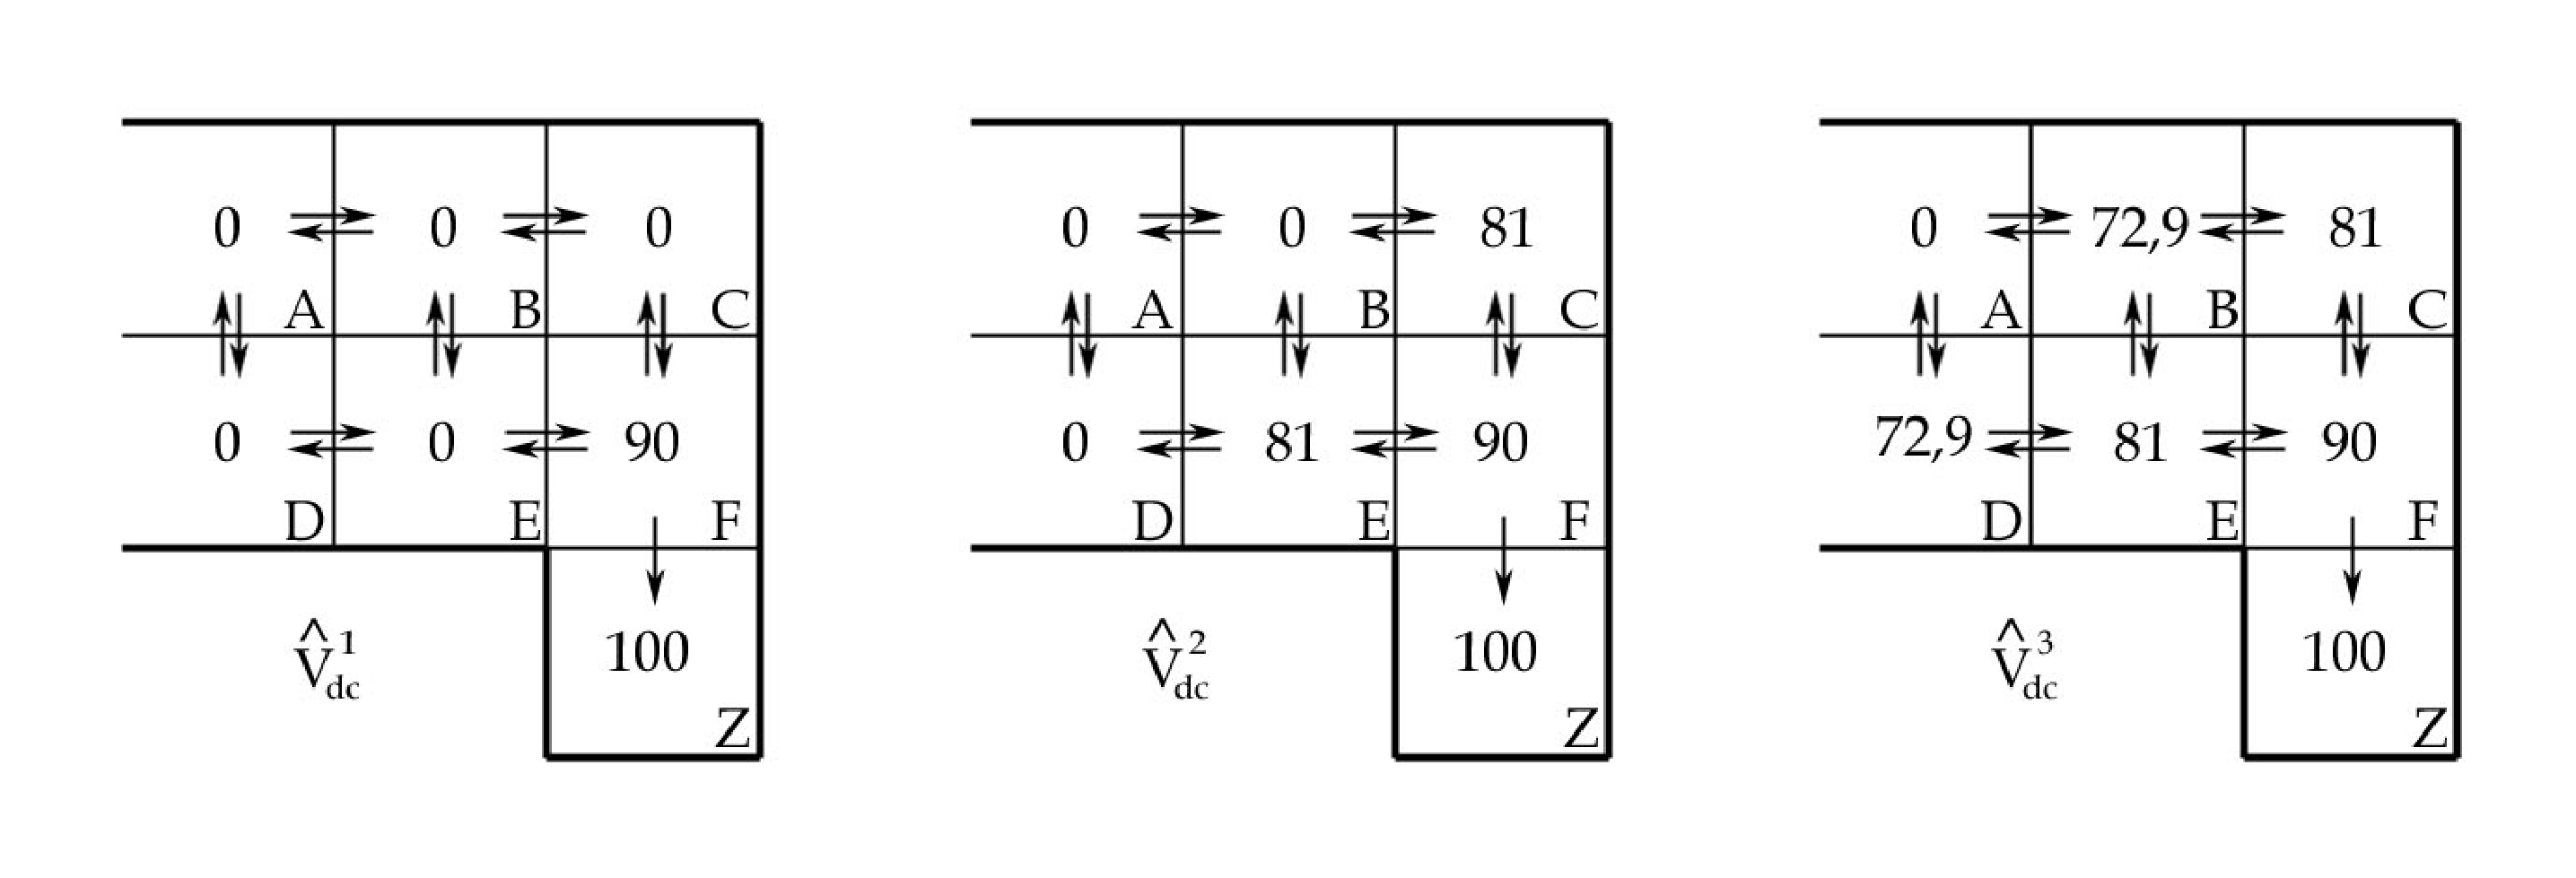
\includegraphics[width=1.0\textwidth]{../images/value_iter_all.eps}
	\caption{Value-Iteration Algorithmus: Drei Iterationsschritte}
	\label{fig:Beispiel-Value-Iteration}
\end{figure}

Die Nachteile des Value-Iteration Algorithmus sind z.B. die erforderlichen 
Kenntnisse der Umwelt, in der sich der Agent bewegt. Wie oben schon 
angesprochen muss in der Lernphase bereits die Zustandsübergangsfunktion 
$\delta(s,a)$ und die Belohnungsfunktion $r(s,a)$ bekannt sein.

Im nächsten Abschnitt wird eine Methode vorgestellt, die den Nachteil von MC 
und DP nicht hat.

\subsection{Temporal Difference Learning}
Methoden des Temporal Difference Learning (TD) aktualisieren Nutzenschätzungen, 
so dass sie mit denen von Nachfolgezuständen übereinstimmen. Hierfür werden 
Ideen der Monte-Carlo-Strategie und die Vorgehensweise des Dynamischen 
Programmierens kombiniert.

\par Man spricht bei dieser Klasse von Lösungsmethoden auch von 
"`modellfreien"' Verfahren, da hierfür kein Modell der Umwelt benötigt wird. 
Das Verfahren des \textbf{Q-Learnings}, das im Folgenden näher behandelt wird, stellt 
eine Unterklasse eben dieser TD-\-Lern\-ver\-fah\-ren dar.

\subsubsection{Q-Learning}
Das Konzept des Q-Lernens ist eine Variante des Temporal Difference Learning 
bzw.\ stellt eine Lösungsstrategie eben genannter Strategie dar.
\par Hierbei ist für das Q-Lernen kein Modell erforderlich, weder in der Lern- 
noch in der Aktionsauswahlphase. Man spricht hier von "`Lernen in unbekannter 
Umgebung"', das heißt konkret, dass weder die Zustandsübergangsfunktion 
$\delta(s,a)$ noch die Belohnungsfunktion (Reward) $r(s,a)$ bekannt sind.
Dies vereinfacht das Problem, schränkt aber möglicherweise die Fähigkeit ein, 
in komplexen Umgebungen zu lernen, weil der Agent die Ergebnisse möglicher 
Aktionsfolgen nicht vorhersehen bzw. simulieren kann.
\par Ziel des Q-Learnings ist das Erlernen einer Aktion-Wert-Funktion 
(Q-Funktion) durch Exploration, die den Nutzen eines Zustandsübergangs durch 
Auswahl einer bestimmten Aktion widerspiegelt.
Diese Aktion-Wert-Funktion liefert hierzu für jeden Zustandsübergang einen 
Nutzenwert $\hat{Q}(s,a)$ einer Aktion $a$ in Zustand $s$ unter Annahme, dass 
danach $\pi^*$ (optimale Policy) folgt. Um den besten Weg (sprich der Weg, der 
den jeweiligen Q-Wert je Zustand maximiert) zu finden, ist die Initialisierung 
aller Q-Werte notwendig. Die optimale Aktion $a^*$ ist somit die mit dem 
aktuell höchsten Q-Wert (Formel siehe weiter unten). Der Lernalgorithmus 
funktioniert nach ähnlichen Prinzip wie der Value-Iteration Algorithmus, 
benutzt aber nur Informationen, an die der Agent durch Ausprobieren von 
Aktionen in seiner Umwelt selber gelangen kann.

\paragraph{Q-Learning Algorithmus [Watkins, 1989]}
\begin{itemize}
  \item Eingabe: Zustände, kurzfristige Rewards $r$.
  \item Ausgabe: Tabelle  $\hat{Q}(s,a)$, die zu jedem Zustand $s$ die optimale 
  Aktion $a^*$ angibt. Daraus lässt sich eine Policy $\pi$ bilden.
  \item Laufzeit: schwierig abzuschätzen, weil Algorithmus konvergiert.
\end{itemize}

\paragraph{Ablauf}
\begin{enumerate}
  \item Initialisiere $\hat{Q}(s,a) = 0$ $\forall$ $s \in S$ und $a \in A$, $s$ 
  ist Startzustand
  \item Wiederhole solange der Agent lebt bzw.\ solange wie Änderungen von Q 
  klein genug sind
  \begin{itemize}
    \item wähle eine Aktion $a$ und führe sie aus bzw. nach Ablauf des ersten
    Iterationsdurchgangs wähle optimale Aktion $a^*$
    \item erhalte kurzfristige Belohnung (Reward) $r \in R$ und neuen Zustand 
    $s' \in S$
    \item $\hat{Q}(s,a) := r + \gamma \cdot max_{a' \in A}\hat{Q}(s',a')$,
    wobei $\gamma$ = Discountfaktor mit  $0 < \gamma < 1$
    \item $s := s'$
  \end{itemize}
  \item Gib optimale Policy  $\pi^*(s) = argmax_{a}\hat{Q}(s,a)$.
\end{enumerate}

Es kann also gezeigt werden, dass die Werte $\hat{Q}(s,a)$ gegen die optimalen 
Q-Werte $Q^*(s,a)$ (sprich gegen die Q-Funktion) nach unendlicher Anzahl an 
Iterationen konvergieren. Nach einer ausreichenden Anzahl an Trainingsschritten 
kann also die optimale Policy berechnet werden, indem für jeden Zustand $s$ die 
optimale Aktion $a^*$ gewählt wird, die $\hat{Q}(s,a)$ maximiert (Greedy-Strategie):

\[ 
a^* = argmax_{a}\hat{Q}(s,a)
\]

Hier in Abbildung \ref{fig:Beispiel-QLearning} ist der Ablauf des Q-Learning 
Algorithmus dargestellt.

\begin{figure}
	\centering
	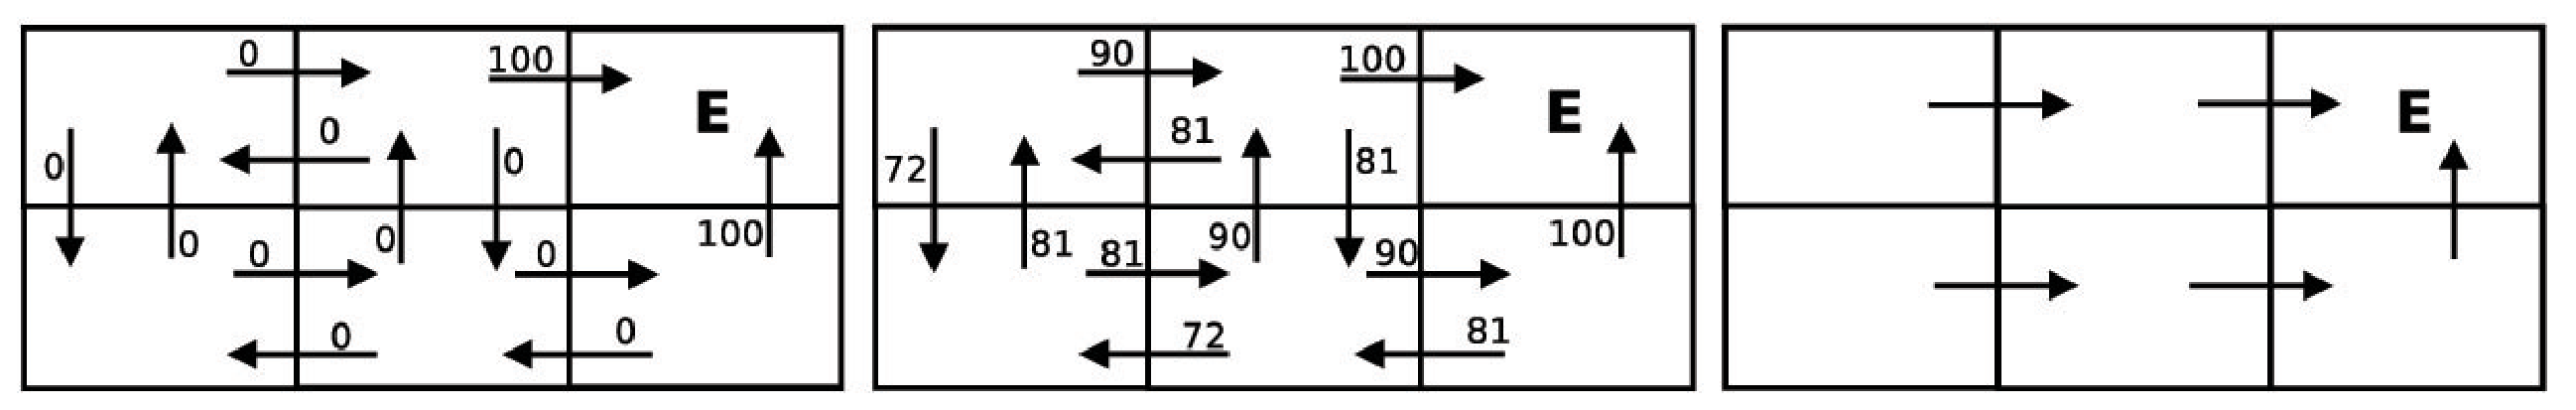
\includegraphics[width=1.0\textwidth]{../images/Q_Policy.eps}
	\caption{Q-Learning Algorithmus: $\hat{Q}(s,a)$-Werte und eine daraus 
	resultierende, optimale policy $\pi^*$}
	\label{fig:Beispiel-QLearning}
\end{figure}

Der Q-Learning Algorithmus besitzt jedoch auch einige Nachteile, z.\,B.\ 
benötigt er viele Iterationsschritte in der Lernphase (Exploration) und dies 
wirkt sich natürlich bei großem Zustandsraum wesentlich auf die Lauf- und Rechenzeit aus.

\subsubsection{Exploration vs. Exploitation}
Selbst wenn sich nach Konvergenz gute und schlechte Verhalten unterscheiden 
lassen, ist noch nicht gewährleistet, dass sich unter den guten Verhalten auch 
das optimale Verhalten befindet. \par Deshalb wird das System im Normalfall 
versuchen, ab und zu neue Verhalten auszuprobieren. Dieses Vorgehen/dieser Modi 
wird als \textbf{Exploration (Erforschung)} bezeichnet. Es wird sich am besten 
bekannten Verhalten orientieren und dies leicht modifizieren, ausüben und dann 
der anschließenden Bewertung zuführen. Wie oft solche Variationen durchgeführt 
werden, kann über einen Zufallsgenerator getriggert werden (d.h. wenn dieser 
unter einem parametrisierbaren Schwellwert liegt). Sollte dieser Schwellwert 
gleich Null sein, erfolgt keinerlei Variation. Dann wird keine weitere 
Optimierung der Verhalten durchgeführt und lediglich das aufgebaute Verhalten 
genutzt. Diesen Modus nennt man \textbf{Exploitation (Ausnutzung)}.

\section{Anwendungsgebiete und Fazit}
Mit Reinforcement-Lernalgorithmen konnten bereits eine Reihe bedeutender 
Probleme gelöst werden, wie z.\,B.\ Backgammon (Tesauro 1994, 1995). \par 
Sutton und Barto analysierten Samuals Mühleprogramm vom Standpunkt des 
Re\-in\-force\-ment-Lernens. Sie stellen zudem unter Verwendung des 
Reinforcement-Ansatzes entwickelte Lösungen für interessante Probleme wie die 
dynamische Kanalzuweisung und die Buchhaltung von Werkstattterminen vor (Sutton 
und Barto 1998).
